\begin{ex}
Uma pessoa vai de A até B andando para cima e para a direita. Qual a probabilidade que passe por C?
\begin{center}
    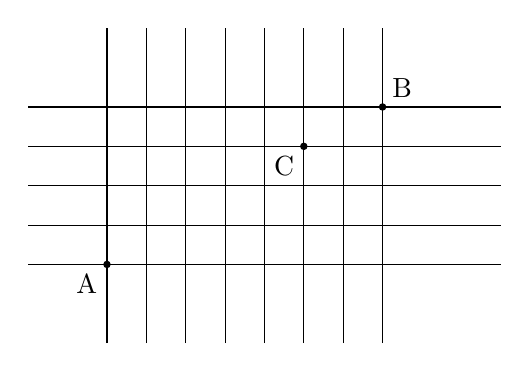
\begin{tikzpicture}
    \draw (-1,0)--(5,0);
    \draw (-1,.5)--(5,.5);
    \draw (-1,1)--(5,1);
    \draw (-1,1.5)--(5,1.5);
    \draw (-1,2)--(5,2);
    \draw (0,-1)--(0,3);
    \draw (.5,-1)--(.5,3);
    \draw (1,-1)--(1,3);
    \draw (1.5,-1)--(1.5,3);
    \draw (2,-1)--(2,3);
    \draw (2.5,-1)--(2.5,3);
    \draw (3,-1)--(3,3);
    \draw (3.5,-1)--(3.5,3);

    \draw[fill] (0,0) circle [radius=0.040];
    \node [below left] at (0,0) {A};

    \draw[fill] (2.5,1.5) circle [radius=0.040];
    \node [below left] at (2.5,1.5) {C};

    \draw[fill] (3.5,2) circle [radius=0.040];
    \node [above right] at (3.5,2) {B};

    \end{tikzpicture}
\end{center}
   \begin{sol}
     \phantom{A}  \\
     de A para B: 7 para a direita e 4 para cima = $\frac{11!}{7!\cdot4!}=330$ \\
     de A para C: 5 para a direita e 3 para cima = $\frac{8!}{5!\cdot3!}=56$  \\
     $p=\frac{56}{330}=\frac{28}{165}$
   \end{sol}


\end{ex}